\documentclass{article}
\usepackage{graphicx}
\usepackage[utf8]{inputenc}
\usepackage{amsmath, amssymb, latexsym}
\usepackage{neuralnetwork}
\usepackage{multicol}

\usepackage{pgfplots}
\usepackage{algorithm}
\usepackage[noend]{algpseudocode}
\usepackage{tikz}
\usepackage{nicefrac}
\pgfplotsset{every axis legend/.append style={
at={(0,0)},
anchor=north east}}
\usetikzlibrary{shapes,positioning,intersections,quotes}
\usetikzlibrary{arrows.meta,
                bending,
                intersections,
                quotes,
                shapes.geometric}
                
\definecolor{darkgreen}{rgb}{0.0, 0.6, 0.0}
\definecolor{darkred}{rgb}{0.7, 0.0, 0.0}
\makeatletter
\def\BState{\State\hskip-\ALG@thistlm}
\makeatother
\title{Week 10}
\begin{document}
\pagenumbering{gobble}
\maketitle
\newpage
\pagenumbering{arabic}

\section*{Debugging a learning algorithm}

Imagine you've used regularized linear regression to forecast home prices:

$$J(\theta) = \frac{1}{2m} [ \sum_{i=1}^{m}(h_{\theta}(x^{(i)} + y^{(i)})^2 + \lambda \sum_{j=1}^{m} \theta_j^2] $$

\begin{itemize}
  \item Trained it.
  \item However, when tested on new data, it produces unacceptably high errors in its predictions.
  \item What should your next step be?
        \begin{itemize}
          \item Obtain additional training data.
          \item Try a smaller set of features.
          \item Consider getting more features.
          \item Add polynomial features.
          \item Change the value of $\lambda$.
        \end{itemize}

\end{itemize}

\section*{Evaluating a hypothesis}

\begin{itemize}
  \item Split data into two portions: training set and test set.
  \item Learn parameters $\theta$ from training data, minimizing $J(\theta)$ using 70\% of the training data.
  \item Compute the test error.

        $$J_{test}(\theta) = \frac{1}{2m_{test}}  \sum_{i=1}^{m_{test}}(h_{\theta}(x^{(i)}_{test} + y^{(i)}_{test})^2$$

\end{itemize}

\section*{Model selection and training validation test sets}

\begin{itemize}
  \item How should a regularization parameter or polynomial degree be chosen?
  \item We've previously discussed the issue of overfitting.
  \item This is why, in general, training set error is a poor predictor of hypothesis accuracy for new data (generalization).
  \item Try to determine the degree of polynomial that will fit data.

        1. $h_{\theta}(x) = \theta_0 + \theta_1x$

        2. $h_{\theta}(x) = \theta_0 + \theta_1x + \theta_2x^2$

        3. $h_{\theta}(x) = \theta_0 + ... + \theta_3x^3$

        \quad \vdots

        10. $h_{\theta}(x) = \theta_0 + ... + \theta_{10}x^{10}$

  \item Introduce a new parameter d, which represents the degree of polynomial you want to use.
  \item Model 1 is minimized using training data, resulting in a parameter vector $\theta^1$ (where d =1).
  \item Same goes for other models up to $n$.
  \item Using the previous formula, examine the test set error for each computed parameter $J_{test}(\theta^k)$.
  \item Minimize cost function for each of the models as before.
  \item Test these hypothesis on the cross validation set to generate the cross validation error.
  \item Pick the hypothesis with the lowest cross validation error.
\end{itemize}

~\\
Training error:
        $$J_{train}(\theta) = \frac{1}{2m}  \sum_{i=1}^{m}(h_{\theta}(x^{(i)} + y^{(i)})^2$$
        
~\\
Cross Validation error:
        $$J_{cv}(\theta) = \frac{1}{2m_{cv}}  \sum_{i=1}^{m_{cv}}(h_{\theta}(x^{(i)}_{cv} + y^{(i)}_{cv})^2$$
        
~\\
Test error:
        $$J_{test}(\theta) = \frac{1}{2m_{test}}  \sum_{i=1}^{m_{test}}(h_{\theta}(x^{(i)}_{test} + y^{(i)}_{test})^2$$

\section*{Model selection and training validation test sets}

Bad results are generally the consequence of one of the following:

\begin{itemize}
  \item High bias - under fitting problem.
  \item High variance - over fitting problem.
\end{itemize}

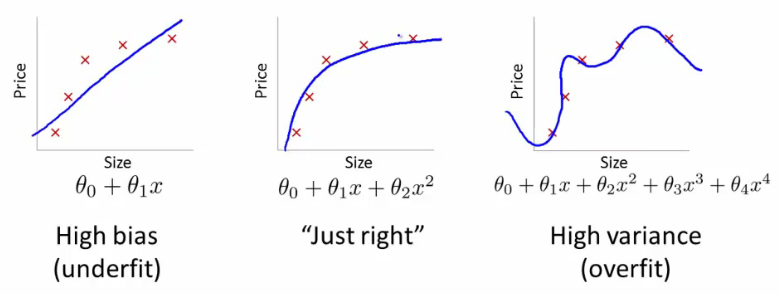
\includegraphics[width=\textwidth]{resources/diagnosis}

Now plot 

\begin{itemize}
  \item $x$ = degree of polynomial d
  \item $y$ = error for both training and cross validation (two lines)
\end{itemize}

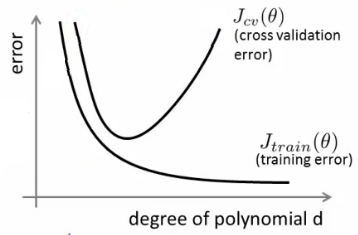
\includegraphics[width=0.5\textwidth]{resources/error_vs_d}

\begin{itemize}
  \item For the high bias case, we find both cross validation and training error are high
  \item For high variance, we find the cross validation error is high but training error is low
\end{itemize}

\section*{Regularization and bias/variance}

Linear regression with regularization:

$$h_{\theta}(x) = \theta_0 + \theta_1x + \theta_2x^2 + \theta_3x^3 + \theta_4x^4$$

$$J(\theta) = \frac{1}{2m} [ \sum_{i=1}^{m}(h_{\theta}(x^{(i)} + y^{(i)})^2 + \lambda \sum_{j=1}^{m} \theta_j^2]$$

The above equation describes the fitting of a high order polynomial with regularization (used to keep parameter values small).

\begin{enumerate}
  \item $\lambda$ is large (high bias $->$ under fitting data)
  \item $\lambda$ is intermediate (good)
  \item $\lambda$ is small (high variance $->$ overfitting)
\end{enumerate}

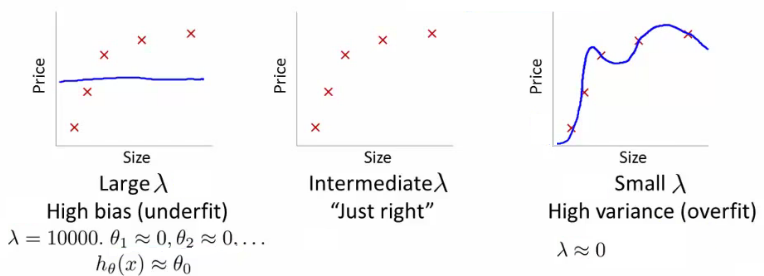
\includegraphics[width=\textwidth]{resources/lambda}

\begin{itemize}
  \item Have a set or range of values to use (for example from 0 to 15).
  \item For each $\lambda_i$ minimize the cost function. Result is  $\theta^{(i)}$.
  \item For each $\theta^{(i)}$ measure average squared error on cross validation set.
  \item Pick the model which gives the lowest error.
\end{itemize}

\section*{Learning curves}

Plot $J_{train}$ (average squared error on training set) and $J_{cv}$ (average squared error on cross validation set) against m (number of training examples).

\begin{itemize}
  \item  $J_{train}$ on smaller sample sizes is smaller (as less variance to accommodate).
  \item  As training set grows your hypothesis generalize better and $J_{cv}$ gets smaller.
\end{itemize}

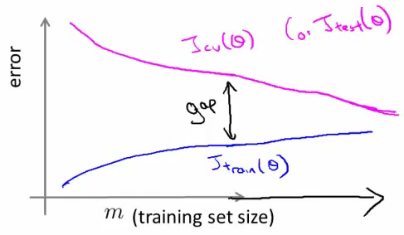
\includegraphics[width=0.6\textwidth]{resources/learning_curve}

\begin{itemize}
  \item  A small gap between training error and cross validation error might indicate high bias. Here, more data will not help.
  \item  A large gap between training error and cross validation error might indicate high variance. Here, more data will probably help.

\end{itemize}

\end{document}